\chap{Der Roboter findet seinen Weg selbst}
\label{ch.line}

Eine Wanderung in den Bergen ist ein einfaches Vorhaben: Nimm dir ein Paar Wanderschuhe und folge dem Pfad. Für einen Roboter, kann das Folgen einer Linie ebenfalls sehr nützlich sein.
Stell Dir ein Lagerhaus mit Roboterwagen vor,
welche Gegenstände von einer zentralen Verteilstelle herbringen.
Dazu werden Linien auf den Boden des Lagerhauses gezeichnet
und die Roboter erhalten die Anweisung bestimmten Linien zu folgen,
bis diese den Lagerplatz für den gewünschten Gegenstand erreichen.
Um dies tun, muss der Roboter diese Linien erkennen können.
Schreibe ein Programm, welches den Roboter einer Linie auf dem Boden folgen lässt.

{\raggedleft \hfill Program file \bu{follow-line.aesl}}

Die Aufgabe "Der Roboter folgt der Linie"  zeigt
alle Unsicherheiten bei der Konstruktion von Robotern in der echten Welt auf.
So kann es sein, dass die Linie zum Beispiel nicht perfekt ist,
Staub kann auf der Linie liegen und diese abdecken,
Dreck führt eventuell dazu, dass ein Rad weniger schnell ist wie das andere.
Damit der Roboter der Linie folgt, benötigt der Roboter eine
\emph{Steuereinheit}, die entscheidet, wieviel Leistung jeder Motor benötigt,
abhängig von den Daten, die von den Sensoren geliefert werden.

\sect{Die Linie und der Roboter}

\begin{figure}
	\subfigure[Thymio folgt einer Klebebandlinie]{ \label{fig.tape} \includegraphics[height=0.35\textwidth]{blacktape}}
	\hfill
	\subfigure[Der linke Sensor ist neben und der rechte Sensor auf dem Klebeband]{ \label{fig.one-off} 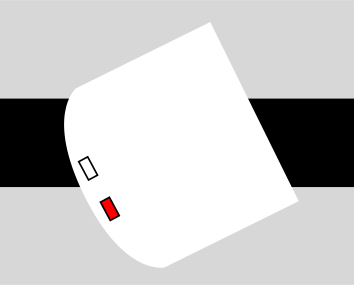
\includegraphics[height=0.35\textwidth]{thymio_half_on_line}}
	\caption{Thymio auf einem schwarzen Klebeband}
\end{figure}
Um der Linie zu folgen, benutzen wir die Bodensensoren (\cref{c.moving}). Erinnere dich daran, dass diese Sensoren durch das Aussenden von Infrarotlicht (unsichtbar für das menschliche Auge) und dem Messen des reflektierten Lichts funktionieren. Falls der Boden von heller Farbe ist,
wird der Sensor viel reflektiertes Licht wahrnehmen und das Ereignis  \blksm{lots-of-light} wird ausgelöst.
Somit brauchen wir eine Linie, die eine Ereignis auslöst, 
falls wenig Licht reflektiert wird \blksm{little-light}.
Das lässt sich einfach mit dem Aufmalen einer schwarzen Linie oder mit dem Anbringen eines schwarzen
Isolierklebebandes auf den Boden bewerkstelligen(\cref{fig.tape}).
Das Klebeband muss breit genug sein,
damit beide Bodensensoren die schwarze Fläche erkennen können,
solange der Roboter erfolgreich dem Klebeband folgt.
Ein Klebeband mit der Breite von 5 Zentimetern genügt dem Roboter,
um dem Klebeband folgen zu können. Die Breite kann auch ein wenig variieren.

Zuerst bringen wir den Roboter dazu,  sich vorwärts zu bewegen,
falls \emph{beide} Sensoren eine dunkle Oberfläche (das schwarze Klebeband) erkennen 
und stoppen, falls \emph{beide} Sensoren eine helle Oberfläche (nicht das Klebeband, sondern den Boden) erkennen.
Die Ereignis-Aktions Paare sind in der folgenden Abbildung \cref{fig.start-stop} gezeigt.

\trickbox{Versichere dich,
dass das USB Kabel lange genug ist (ca. 2m),
damit der Thymio auch in Bewegung mit dem Computer verbunden bleibt. Verlängerungskabel findest du in jedem Computershop.}

\begin{figure}
	\subfigure[Starte und stoppe den Roboter]{ \label{fig.start-stop} \includegraphics[width=0.4\textwidth]{line-forward}}
	\hfill
	\subfigure[Korrektur der Richtungsabweichung]{ \label{fig.follow-line} \includegraphics[width=0.4\textwidth]{line-controller}}
	\caption{Ein Programm, um der Linie zu folgen}
\end{figure}

\sect{Deine erste Steuerungseinheit}

Der nächste Schritt besteht im Programmieren der Steuerungseinheit,
die den Roboter der Linie folgen lässt.

\begin{itemize}

\item Falls der Roboter nach der \emph{linken} Seite vom Klebeband abkommt,
wird der \emph{linke} Sensor den Boden erkennen,
während der \emph{rechte} Sensor immer noch das Klebeband erkennt.
In diesem Fall soll der Roboter ein wenig nach \emph{rechts} abbiegen

\item Falls der Roboter nach der \emph{rechten} Seite vom Klebeband abkommt,
wird der \emph{rechte} Sensor den Boden erkennen,
während der \emph{linke} Sensor immer noch das Klebeband erkennt.
In diesem Fall soll der Roboter ein wenig nach \emph{links} abbiegen.
\end{itemize}

Zwei Ereignis-Aktions Paare werden gebraucht  (Figure~\ref{fig.follow-line}).

\sect{Setzen der Parameter}

Es ist einfach zu erkennen,
dass der Roboter, falls er von der linken Seite des Klebebands abkommt,
wie in Abbildung (Figure~\ref{fig.follow-line}) nach rechts drehen muss,
aber wie weit nach rechts? Falls die Drehung zu gering ausfällt,
wird der rechte Sensor eventuell \emph{auch} vom Klebeband abkommen,
bevor der Roboter auf die Spur zurückgelangt.
Falls der Roboter jedoch zu stark nach rechts dreht,
riskiert der Roboter die Klebeband Spur auf der anderen Seite zu verlieren.
In jedem Fall sind starke Drehungen gefährlich für den Roboter und jegliches Gut,
welches er transportiert.

In diesem Programm können die Geschwindigkeiten des linken und des rechten Motors auf jedem Aktionsblock der Motoren verändert werden.
Experimentiere solange mit diesen Werten,
bis der Roboter \emph{zuverlässig} läuft.
Zuverlässig heisst hier, dass der Roboter mit denselben Programmeinstellungen mehrmals erfolgreich der Linie folgt.
Platziere bei jedem Versuch den Roboter ein wenig anders in Bezug auf die Richtung und Position zum Klebeband.
Das Programm muss mehrmals getestet werden, um die Zuverlässigkeit zu überprüfen.

Es gibt viele Arten, wie die Motorenaktionsblöcke eingestellt werden können, um die Drehung zu kontrollieren, damit der Roboter auf der Linie bleibt. Die vorwärtsgerichtete Geschwindigkeit entlang des Klebebands ist eine wichtige Einflussgrösse (Parameter). 
Ist der Roboter zu schnell,
ist dieser schon vom Klebeband weggefahren,
bevor die Drehbewegung die Richtung des Roboters verändern konnte.
Ist der Roboter jedoch zu langsam, wird dir natürlich niemand deinen Roboter abkaufen
und in einem Lagerhaus einsetzen.

Was soll Thymio tun, falls er von der Linie fährt?
Falls er eine enge Kurfe fährt (dazu kannst du einen Motor vorwärts und den Anderen rückwärts laufen lassen), findet der Roboter rasch zur Linie zurück, die Bewegung des Roboters wird jedoch ruckartig. Andererseits, wenn der Roboter nur eine leichte Drehung vollführt (dazu kannst du den einen Motor etwas schneller als den Anderen laufen lassen), wird der Roboter sich zwar flüssig bewegen, eventuell jedoch die Linie verlieren. Experimentiere, bis du einen guten Kompromiss gefunden hast.


\exercisebox{\thechapter.1}{
Der Roboter stoppt,
falls beide Sensoren erkennen,
dass sie vom Klebeband abgekommen sind.
Verändere das Programm so,
dass der Roboter eine geringe Drehung nach links vollführt mit der Absicht das Klebeband wiederzufinden.
Versuche es auf einem Klebeband mit einer Linkskurve,
wie in der Abbildung \cref{fig.tape} angezeigt.
Versuche die Vorwärtsgeschwindigkeit des Roboters zu erhöhen.
Was passiert, wenn der Roboter das Ende des Klebebandes erreicht hat?
}

\vfill

\exercisebox{\thechapter.2}{
Verändere das Programm aus der vorangehenden Übung so,
dass der Roboter nach rechts dreht,
falls er vom Klebeband abkommt.
Was passiert?
Es wäre wünschenswert,
wenn der Roboter \emph{sich erinnern} könnte,
welchen Sensor als letzter den Kontakt zum Klebeband verloren hat,
um den Roboter in die korrekte Richtung zu führen,
um das Klebeband wieder zufinden.
In Kapitel ~\cref{ch.states} werden wir lernen,
wie Informationen gespeichert werden können.
}

\vfill

\exercisebox{\thechapter.3}{
Experimentiere mit unterschiedlichen Anordnungen des Klebebandes:
\begin{itemize}
\item weiten Kurven
\item engen Kurven
\item zickzack Linien
\item breiteren Linien (benutze dazu die doppelte Klebebandbreite)
\item schmaleren Linien (schneide dazu das Klebeband in zwei Hälften)
\end{itemize}
Veranstalte mit deinen Freunden Roboterrennen:
Welcher Roboter folgt erfolgreich den meisten Linien?
Welcher Roboter fährt am schnellsten eine Linie ab?
}

\vfill

\exercisebox{\thechapter.4}{
Bespreche den Effekt der folgenden Veränderungen  auf den Thymio Roboter und dessen Fähigkeit der Linie zu folgen.
\begin{itemize}
\item Die Messereignisse der Bodensensoren erfolgen öfters bzw. weniger oft als 10 Mal pro Sekunde.
\item Die Sensoren sind weiter auseinander bzw. näher beisammen.
\item Es gibt mehr als zwei Bodensensoren am Boden des Roboters.
\end{itemize}
}